\documentclass{article}

% if you need to pass options to natbib, use, e.g.:
\PassOptionsToPackage{numbers, compress}{natbib}
% before loading neurips_2025

% The authors should use one of these tracks.
% Before accepting by the NeurIPS conference, select one of the options below.
% 0. "default" for submission
 \usepackage{neurips_2025}
% the "default" option is equal to the "main" option, which is used for the Main Track with double-blind reviewing.
% 1. "main" option is used for the Main Track
%  \usepackage[main]{neurips_2025}
% 2. "position" option is used for the Position Paper Track
%  \usepackage[position]{neurips_2025}
% 3. "dandb" option is used for the Datasets & Benchmarks Track
 % \usepackage[dandb]{neurips_2025}
% 4. "creativeai" option is used for the Creative AI Track
%  \usepackage[creativeai]{neurips_2025}
% 5. "sglblindworkshop" option is used for the Workshop with single-blind reviewing
 % \usepackage[sglblindworkshop]{neurips_2025}
% 6. "dblblindworkshop" option is used for the Workshop with double-blind reviewing
%  \usepackage[dblblindworkshop]{neurips_2025}

% After being accepted, the authors should add "final" behind the track to compile a camera-ready version.
% 1. Main Track
 % \usepackage[main, final]{neurips_2025}
% 2. Position Paper Track
%  \usepackage[position, final]{neurips_2025}
% 3. Datasets & Benchmarks Track
 % \usepackage[dandb, final]{neurips_2025}
% 4. Creative AI Track
%  \usepackage[creativeai, final]{neurips_2025}
% 5. Workshop with single-blind reviewing
%  \usepackage[sglblindworkshop, final]{neurips_2025}
% 6. Workshop with double-blind reviewing
%  \usepackage[dblblindworkshop, final]{neurips_2025}
% Note. For the workshop paper template, both \title{} and \workshoptitle{} are required, with the former indicating the paper title shown in the title and the latter indicating the workshop title displayed in the footnote.
% For workshops (5., 6.), the authors should add the name of the workshop, "\workshoptitle" command is used to set the workshop title.
% \workshoptitle{WORKSHOP TITLE}

% "preprint" option is used for arXiv or other preprint submissions
 % \usepackage[preprint]{neurips_2025}

% to avoid loading the natbib package, add option nonatbib:
%    \usepackage[nonatbib]{neurips_2025}

\usepackage[utf8]{inputenc} % allow utf-8 input
\usepackage[T1]{fontenc}    % use 8-bit T1 fonts
\usepackage{hyperref}       % hyperlinks
\usepackage[table]{xcolor}
\usepackage{url}            % simple URL typesetting
\usepackage{booktabs}       % professional-quality tables
\usepackage{amsmath, amssymb, amsfonts}       % blackboard math symbols
\usepackage{nicefrac}       % compact symbols for 1/2, etc.
\usepackage{microtype}      % microtypography
\usepackage{xcolor}         % colors



\usepackage{graphicx}    % For \rotatebox
\usepackage{adjustbox}   % For scaling the table to fit page width
\usepackage{array}       % For column formatting
\usepackage{multirow}    % For multi-row cells
\usepackage{placeins}



% User-defined commands from the prompt - Retained
\newcommand{\Tref}{T_{\text{ref}}}
\newcommand{\Tgen}{T_{\text{gen}}}
\newcommand{\SaT}{\text{SaT}} % Placeholder, define as needed
\newcommand{\nvEmbed}{\text{nvEmbed}} % Placeholder, define as needed
\newcommand{\EmbedNVTwo}{\text{EmbedNV2}} % Placeholder, define as needed
\newcommand{\UOS}{\text{UoS}} % Placeholder, define as needed
\newcommand{\Sref}{S_{\text{ref}}}
\newcommand{\Sgen}{S_{\text{gen}}}
\newcommand{\Cref}{C_{\text{ref}}}
\newcommand{\Cgen}{C_{\text{gen}}}
\newcommand{\Rw}{R_{\mathrm{w}}}
\newcommand{\ECref}{E_{C_{\text{ref}}}}
\newcommand{\ECgen}{E_{C_{\text{gen}}}}
\newcommand{\Nref}{N_{\text{ref}}}
\newcommand{\Ngen}{N_{\text{gen}}}
\newcommand{\D}{D} % dimension
\newcommand{\Erefvec}{\mathbf{E}_{\text{ref}}} % Changed from \Eref to avoid conflict with amsmath
\newcommand{\Egenvec}{\mathbf{E}_{\text{gen}}} % Changed from \Egen to avoid conflict with amsmath
\newcommand{\ciref}{c_{i}^{\text{ref}}}
\newcommand{\cjgen}{c_{j}^{\text{gen}}}
\newcommand{\MWprec}{\text{MW}_{\text{prec}}}
\newcommand{\MWrec}{\text{MW}_{\text{rec}}}
\newcommand{\Mj}{M_j}
\newcommand{\MP}{M_P}
\newcommand{\MR}{M_R}
\newcommand{\LAS}{\text{LAS}}
\newcommand{\LASP}{\text{LAS}_P}
\newcommand{\LASR}{\text{LAS}_R}
\newcommand{\Sim}{\text{Sim}}
\newcommand{\NAS}{\text{NAS}}
\newcommand{\NASD}{\text{NAS}_D}
\newcommand{\NASL}{\text{NAS}_L}
\newcommand{\dprime}{d''}
\newcommand{\Ptotalx}{P_{\text{total},x}}
\newcommand{\Pmaxx}{P_{\text{max},x}}
\newcommand{\NASDP}{\text{NAS}_{DP}}
\newcommand{\NASDR}{\text{NAS}_{DR}}
\newcommand{\Lflooridealx}{L_{\lfloor\text{ideal}\rfloor,x}}
\newcommand{\Lceilidealx}{L_{\lceil\text{ideal}\rceil,x}}
\newcommand{\Lactualx}{L_{\text{actual},x}}
\newcommand{\NASLP}{\text{NAS}_{LP}}
\newcommand{\NASLR}{\text{NAS}_{LR}}
\newcommand{\tauLCT}{\tau_{\text{LCT}}}
\newcommand{\NASFone}{\text{NAS}_{F1}}
\newcommand{\RW}{R_W}
\newcommand{\Atotalmw}{A_{\text{total\_mw}}}
\newcommand{\Atimeline}{A_{\text{timeline}}}
\newcommand{\Aminratio}{A_{\text{min\_ratio}}}
\newcommand{\NASintermediate}{\text{NAS}_{\text{intermediate}}}
\newcommand{\NASinterim}{\text{NAS}_{\text{interim}}}
\newcommand{\NASreg}{\text{NAS}_{\text{reg}}}
\newcommand{\GASLAS}{\text{GAS}_{\text{LAS}}}
\newcommand{\SAS}{\text{SAS}}
\newcommand{\VCSshort}{\text{VCS}_{\text{short}}}
\newcommand{\GAS}{\text{GAS}}

% Note. For the workshop paper template, both \title{} and \workshoptitle{} are required, with the former indicating the paper title shown in the title and the latter indicating the workshop title displayed in the footnote. 
\title{Video Comprehension Score $(VCS)$: A Metric for Long-Form Video Description Evaluation}


% The \author macro works with any number of authors. There are two commands
% used to separate the names and addresses of multiple authors: \And and \AND.
%
% Using \And between authors leaves it to LaTeX to determine where to break the
% lines. Using \AND forces a line break at that point. So, if LaTeX puts 3 of 4
% authors names on the first line, and the last on the second line, try using
% \AND instead of \And before the third author name.


\author{%
  David S.~Hippocampus\thanks{Use footnote for providing further information
    about author (webpage, alternative address)---\emph{not} for acknowledging
    funding agencies.} \\
  Department of Computer Science\\
  Cranberry-Lemon University\\
  Pittsburgh, PA 15213 \\
  \texttt{hippo@cs.cranberry-lemon.edu} \\
  % examples of more authors
  % \And
  % Coauthor \\
  % Affiliation \\
  % Address \\
  % \texttt{email} \\
  % \AND
  % Coauthor \\
  % Affiliation \\
  % Address \\
  % \texttt{email} \\
  % \And
  % Coauthor \\
  % Affiliation \\
  % Address \\
  % \texttt{email} \\
  % \And
  % Coauthor \\
  % Affiliation \\
  % Address \\
  % \texttt{email} \\
}


\begin{document}


\maketitle

\begin{figure}[ht] % You can adjust placement options like [htbp]
  \centering
  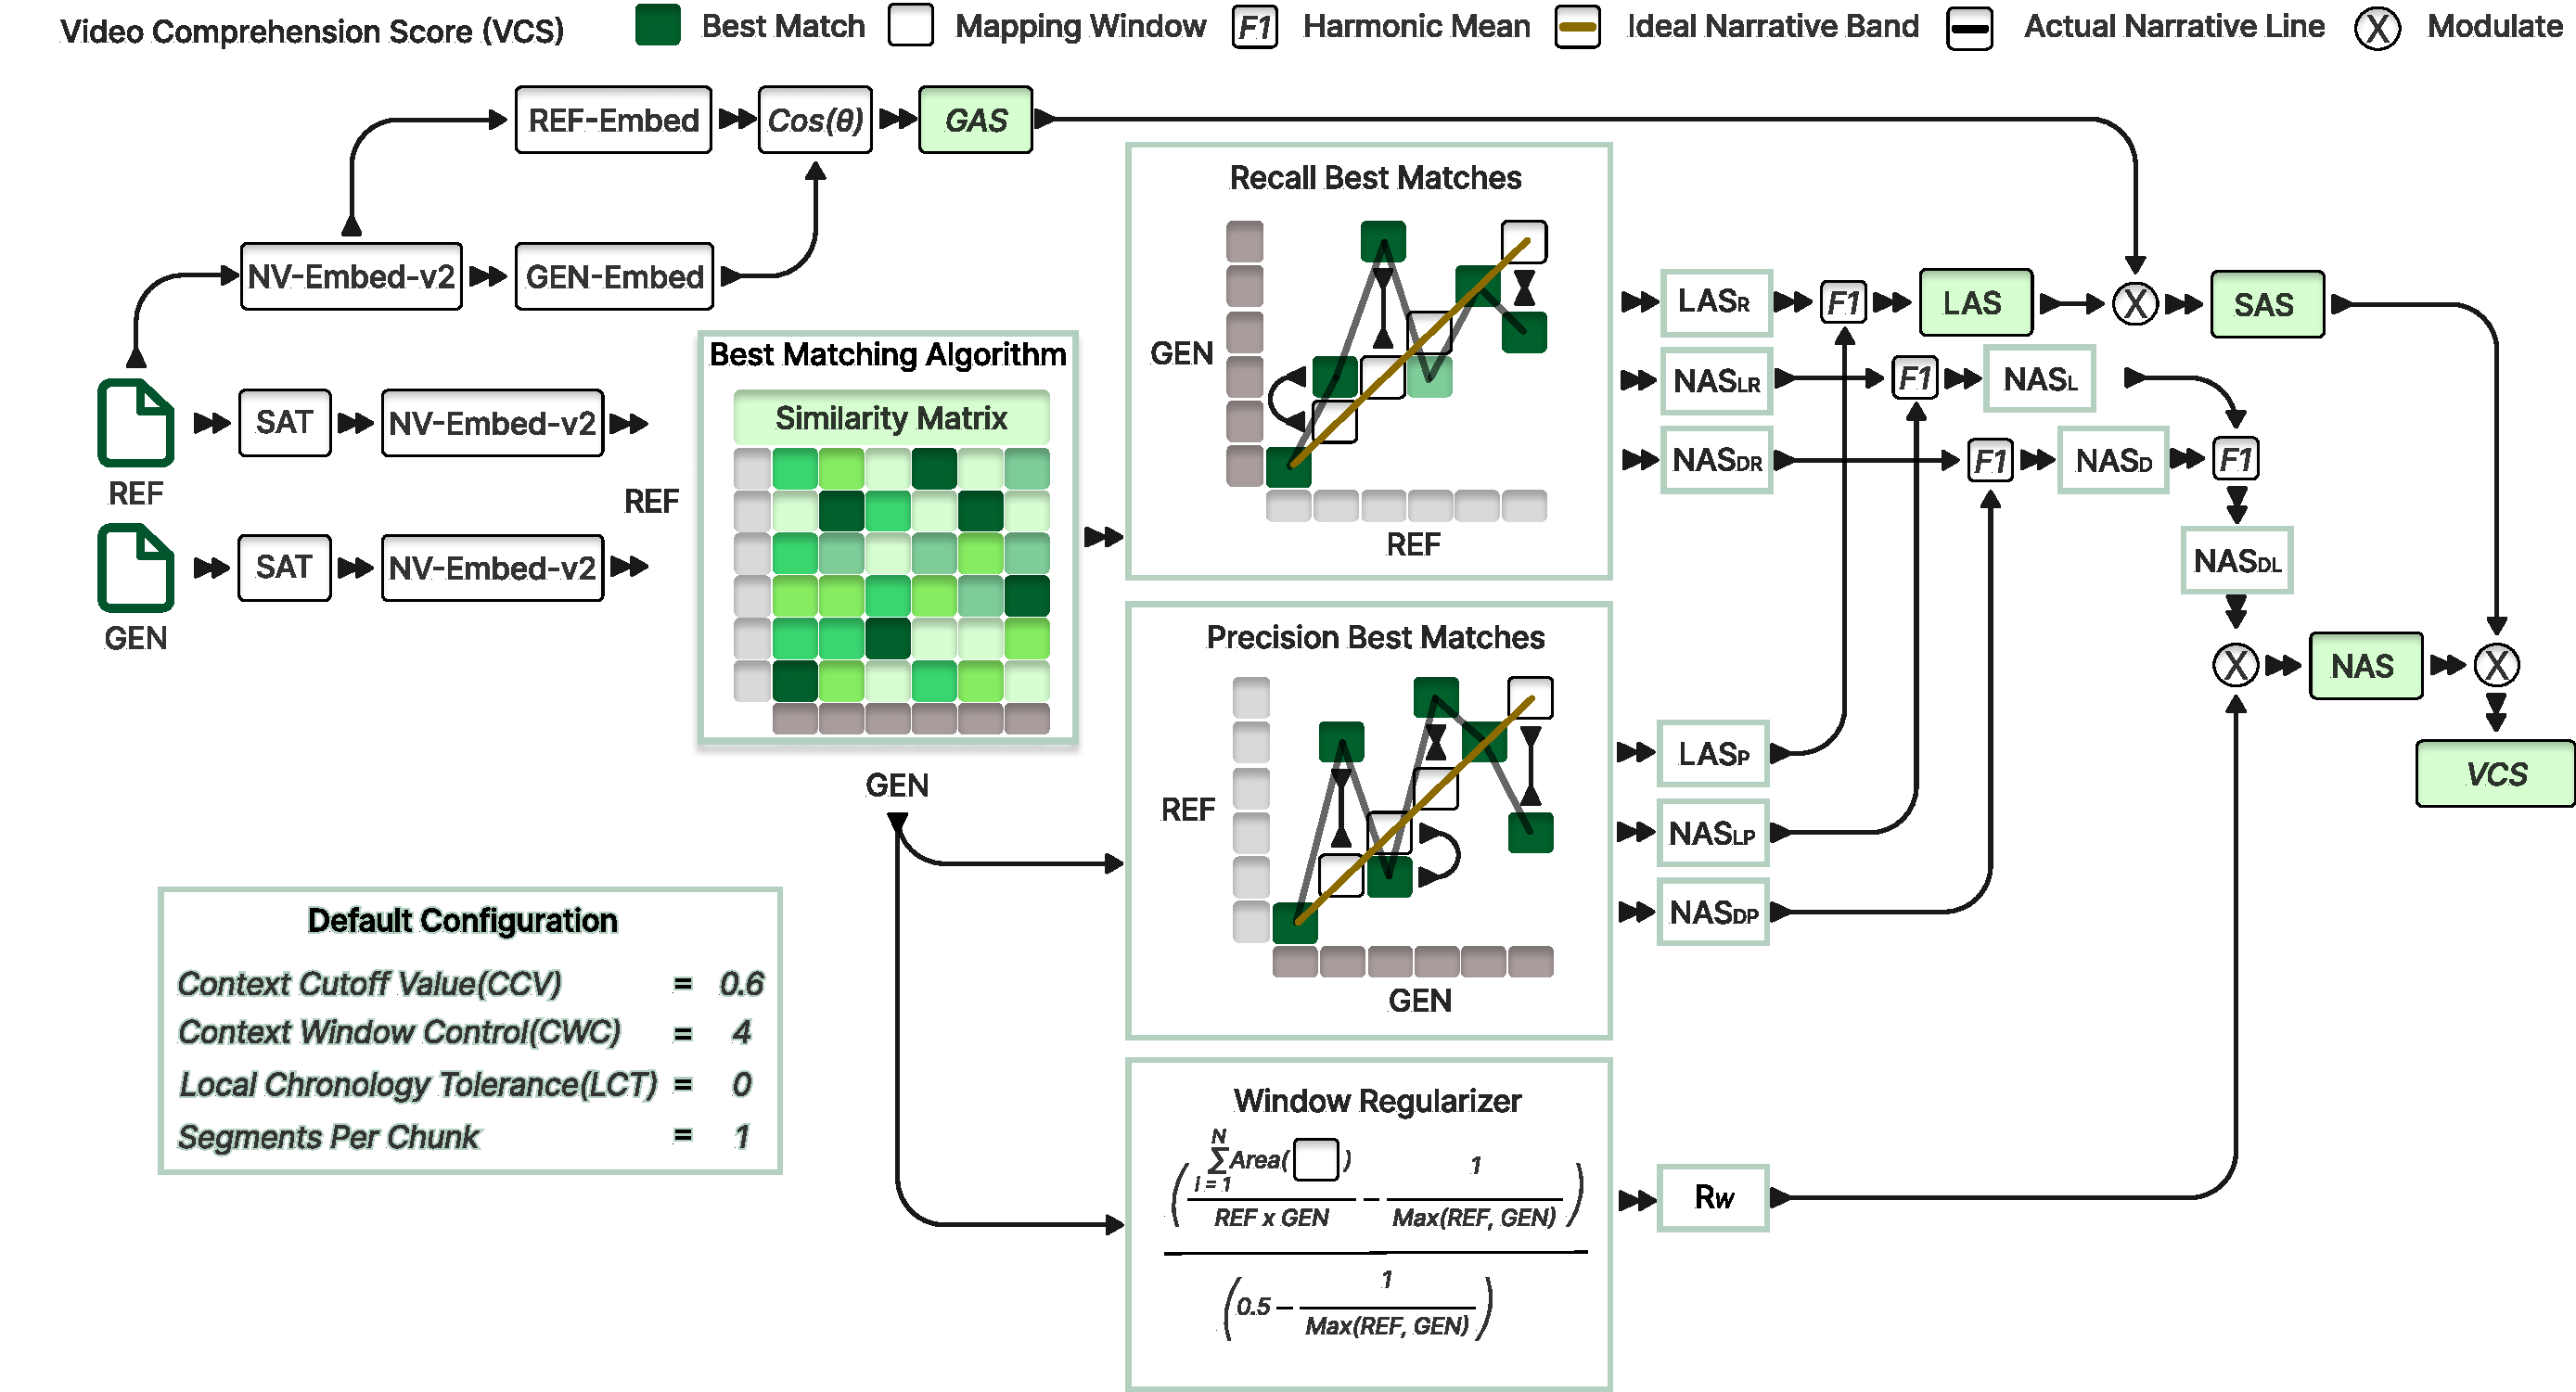
\includegraphics[width=1\textwidth]{VCS.pdf} % Adjust width as needed, or use other options like scale, height.
    \caption{Architecture of the Video Comprehension Score (VCS). The VCS assesses video descriptions by comparing a reference text ($T_{ref}$) with a model-generated text ($T_{gen}$). Both texts are initially segmented by SaT and embedded via nvEmbed. The Global Alignment Score (GAS) is computed from the full text embeddings. For localized analysis, texts are chunked and embedded, forming a similarity matrix. From this, precision and recall-oriented best matches yield the Local Alignment Score (LAS)—the harmonic mean of $LAS_P$ (precision) and $LAS_R$ (recall). The Narrative Alignment Score (NAS) incorporates distance-based ($NAS_D$) and line-based ($NAS_L$) assessments. $NAS_D$ and $NAS_L$ are harmonic means of their respective precision and recall components. A Window Regularizer ($R_w$) refines the NAS. The Semantic Alignment Score (SAS) is derived by modulating GAS with LAS. The final VCS results from modulating the smaller of SAS and the regularized NAS with the larger.}
  \label{fig:VCS} % Optional: for cross-referencing the figure in your text
\end{figure}

\begin{abstract}
    We introduce Video Comprehension Score (VCS), a novel metric for evaluating long-form video comprehension models by comparing generated long video descriptions against human-written references. Current evaluation metrics, including BLEU, ROUGE, METEOR, and CIDEr, rely primarily on rigid text-level comparisons, overlooking narrative coherence, temporal accuracy, and semantic equivalence. Moreover, existing LLM-based metrics such as Auto-DQ and VAD score are computationally expensive and lack sensitivity to event chronology, further complicating accurate evaluation. To address these limitations, VCS employs a unified semantic and temporal framework comprising three key components: Global Alignment Score (GAS), which assesses holistic narrative consistency; Local Alignment Score (LAS), which measures semantic alignment at the segment level; and Narrative Alignment Score (NAS), explicitly capturing temporal correctness. All components utilize robust nv-embed-v2 embeddings, ensuring precise and flexible evaluation from a single human reference. We validate VCS empirically using a synthetic MPII-based dataset containing both valid and invalid narrative variants. VCS significantly outperforms baseline metrics by clearly differentiating correct from incorrect paraphrases, achieving margins exceeding 15 percentage points. Additionally, VCS demonstrates state-of-the-art performance in short-caption evaluations on the VATEX benchmark, attaining the highest human correlation in the 9-reference setting (Kendall $\tau_b=41.5$, Spearman $\rho=51.8$) and competitive results in the single-reference scenario, highlighting its broad applicability and effectiveness.
\end{abstract}

\section{Introduction}

Recent advancements in Large Video Language Models (LVLMs) have significantly advanced automated video understanding, enabling the generation of detailed, long-form narratives from complex video content \cite{he2024ma, chen2024far, achiam2023gpt, cheng2024videollama, ataallah2024goldfish, li2024llava, liu2024st, zhang2023video, lin2023video, ye2024mplug, yao2024minicpm}. This capability is essential for applications demanding nuanced interpretation, including autonomous and assistive technologies. However, effectively evaluating if these models genuinely comprehend a video's narrative—events, entities, and interactions—remains challenging.

Current evaluation often relies on isolated fact-based question-answering tasks \cite{zhou2024mlvu, tapaswi2016movieqa, wang2024lvbench, ataallah2024goldfish, fu2024video,li2024llava, nagrani2024neptune, li2024mvbench, rawal2024cinepile, ataallah2024infinibench, wu2024longvideobench, tan2025allvb}, which inadequately assess holistic comprehension. Traditional n-gram metrics (BLEU, METEOR, CIDEr, ROUGE, SPICE) \cite{papineni2002bleu, banerjee2005meteor, vedantam2015cider, lin2004rouge, anderson2016spice} suffer from the "many-to-one mapping" problem, penalizing stylistic and semantic variations by relying on lexical overlap, and inadequately evaluating narrative chronology. Though consensus-based solutions address the many-to-one mapping issue, generating extensive diverse references for long videos is prohibitively labor-intensive and impractical.

Embedding-based metrics (e.g., BERTScore \cite{zhang2019bertscore}) improve semantic awareness but struggle with context limitations and structural complexity in evaluating lengthy narratives. Recent LLM-driven methods \cite{wang2024tarsier, dubey2025leveraging, maaz2023video} offer semantic nuance but depend heavily on LLM accuracy and suffer from consistency and transparency issues. Critically, these methods often inadequately assess narrative structure and chronology.

Comprehensively scoring dense video narratives involves several interconnected challenges: (1) Many-to-one mapping, exacerbated by practical limitations in generating extensive human annotations. (2) Reconciling strict versus lenient content alignment—allowing valid descriptive variability, such as different event granularities or descriptive styles, while penalizing core distortions. (3) Balancing local chronology tolerance (flexibility in concurrent events or minor reordering) with intolerance (strict ordering of critical sequences). (4) Integrating global and local narrative assessments to detect significant structural misorderings despite locally correct segments, and vice versa.

This paper introduces the Video Comprehension Score (VCS), a novel metric addressing these complexities by evaluating dense, long-form video descriptions semantically and structurally. VCS employs Segment Any Text (\SaT) \cite{frohmann2024segment} for semantic segmentation and $\nvEmbed$ \cite{lee2024nv} for chunk-level embeddings, comprising three components:

\begin{enumerate}
\item Global Alignment Score (GAS): Measures overall thematic similarity using full-text embeddings.
\item Local Alignment Score (LAS): Assesses fine-grained semantic correspondence between chunks.
\item Narrative Alignment Score (NAS): Evaluates chronological consistency, using a configurable LOCAL CHRONOLOGY Tolerance factor (LCT) to balance descriptive flexibility and strict narrative order.
\end{enumerate}

We combine GAS and LAS into a Semantic Alignment Score (SAS), representing semantic alignment across long paragraphs. Integrating SAS with NAS yields the comprehensive VCS metric, enabling clear assessment of narrative equivalence and comprehension between model-generated and human-written descriptions.

Additionally, we generalized VCS to $\VCSshort$, applying the same principles at varying segment lengths, demonstrating its versatility for shorter captions.

Due to the absence of suitable annotated datasets for long-form dense descriptions—where human judgment becomes increasingly unreliable—we constructed a large-scale synthetic dataset (1390 descriptions, ~500 words each, from MPII via ChatGPT) \cite{rohrbach2015dataset, achiam2023gpt}. Two test sets, a Comparison Test Set (27,800 description pairs with diverse valid/invalid variations) and a Multiple-Author Test Set (5560 variants from four LLMs), comprehensively evaluate VCS performance.

Benchmarked against traditional and adapted segment-based metrics (BLEU-S, METEOR-S, ROUGE-L-S), VCS consistently demonstrated robustness to valid narrative variability and sensitivity to invalid alterations. On VATEX-EVAL \cite{shi2022emscore}, $\VCSshort$ achieved state-of-the-art results in the 9-reference setting and was a close second in the 1-reference setting \cite{sarto2023positive}.

The results affirm VCS as a reliable metric capable of accurately assessing narrative equivalence across diverse descriptive styles and lengths, configurable for varying chronological rigor. In summary, our primary contributions include:

\begin{itemize}
\item A versatile, robust metric (VCS) for evaluating dense and diverse video descriptions across varying lengths and styles.
\item A configurable approach to balance semantic and chronological evaluation, adaptable to multiple applications.
\end{itemize}
\section{Related Works}

Traditional n-gram-based metrics such as BLEU \cite{papineni2002bleu}, ROUGE \cite{lin2004rouge}, and METEOR \cite{banerjee2005meteor} evaluate text generation through lexical overlap and local word order. BLEU measures n-gram precision with brevity penalties, capturing local chronology but limited by rigid lexical matching. ROUGE variants emphasize recall; ROUGE-N evaluates n-gram overlap, while ROUGE-L utilizes the Longest Common Subsequence (LCS) at sentence-level, yet remains sensitive to lexical variation and sentence-length discrepancies. METEOR integrates lexical alignment via synonyms and stems, computing precision-recall harmonics with fragmentation penalties for local word order. CIDEr \cite{vedantam2015cider} addresses lexical variability by consensus-based TF-IDF weighting across multiple references but proves impractical for dense, long descriptions due to labor-intensive annotation. SPICE \cite{anderson2016spice} evaluates semantic propositions using graph overlaps, effectively handling paraphrasing but neglecting fluency, grammar, and narrative chronology critical for video descriptions.

Embedding-based metrics compare texts in semantic vector spaces, leveraging pretrained models to capture semantic similarity beyond lexical matches. Early methods like BERTScore \cite{zhang2019bertscore}, MoverScore \cite{zhao2019moverscore}, and SBERT \cite{reimers2019sentence} recognize paraphrases but are constrained by limited context windows, complicating their direct application to extended narratives. Recent decoder-based models (e.g., nv-embed-v2 \cite{lee2024nv}, Linq-Embed-Mistral \cite{choi2024linq}, SFR-Embedding-Mistral \cite{meng2024sfrembedding}, Jasper and Stella \cite{zhang2024jasper}) offer significantly larger context windows and robust global embeddings, excelling at paragraph-level semantic assessments. However, reliance on global embeddings and cosine similarity overlooks local content alignment, detailed information accuracy, and chronological coherence, allowing subtle inaccuracies or misordered events to remain undetected.

Multimodal embedding metrics like EMScore \cite{shi2022emscore} and PAC-S \cite{sarto2023positive} employ vision-language models (e.g., CLIP \cite{radford2021learning}) to evaluate semantic alignment between visuals and generated captions. EMScore combines coarse and fine-grained multimodal matches for accurate short-caption evaluation, whereas PAC-S, fine-tuned via contrastive learning, closely aligns with human judgments. Despite their effectiveness in short-form tasks, these metrics face computational challenges and methodological limitations when scaling to dense, extended narratives, struggling with complex chronology and segment-level coherence without significant adaptations.

Recent evaluation approaches increasingly leverage Large Language Models (LLMs), categorized into component-based and holistic judge methods. Component-based methods (e.g., AutoDQ \cite{wang2024tarsier}, VAD-Score \cite{dubey2025leveraging}) use LLMs for semantic extraction and entailment checks, effectively addressing semantic variation and many-to-one mapping challenges; however, they do not evaluate chronology of events. Nonetheless, their effectiveness depends heavily on extraction accuracy, consistency across model updates, scalability with dense content, and reliance on comprehensive references. Conversely, holistic methods (e.g., ChatGPT-based scoring \cite{achiam2023gpt}) provide overall quality assessments directly from LLMs, theoretically addressing complex evaluation dimensions comprehensively. However, they suffer from ambiguity in score calibration, sensitivity to prompting nuances, consistency issues across model versions, limited interpretability, and practical constraints including reproducibility and cost.


\section{Methodology: Video Comprehension Score (VCS)} % From template

\label{sec:methodology_vcs} % Add a label for the main section if you like

Figure~\ref{fig:VCS} illustrates the overall architecture of the Video Comprehension Score (VCS), a metric designed for the comprehensive evaluation of dense, long-form video descriptions. VCS assesses the quality of model-generated text ($\Tgen$) against a reference text ($\Tref$) by quantifying both semantic and narrative alignment. This approach aims to surpass traditional n-gram-based metrics by specifically addressing challenges such as the "many-to-one mapping" problem and the critical aspect of event ordering for narrative coherence. The subsequent subsections detail the fundamental components, preprocessing techniques, and the suite of metrics that constitute the VCS.

\subsection{Fundamental Components and Preprocessing} % From template
\label{sec:fundamental_components_revised} % From new text
\subsubsection{Core Technologies: Segmentation and Embedding} % From template
\label{ssec:core_technologies_revised} % From new text
VCS employs two core technologies. \SaT\ \cite{frohmann2024segment} segments texts into granular semantic segments for robust comparison of potentially noisy inputs. Subsequently, $\nvEmbed$\cite{lee2024nv} converts textual units (full texts and chunks) into high-dimensional vector embeddings, enabling quantitative similarity measurement.

\subsubsection{Text Preprocessing: Segmentation and Chunking for VCS} % Title from new text (more specific)
\label{sssec:text_preprocessing_and_chunking_revised} % From new text
For standard VCS (long-form descriptions), input texts $\Tref$ and $\Tgen$ are cleaned, typically involving removal of punctuation and full stops. \SaT\ \cite{frohmann2024segment} then segments these into sequences of semantic segments, $\Sref$ and $\Sgen$. To balance granularity and context, $k$ consecutive segments form "chunks," resulting in sequences $\Cref$ and $\Cgen$. These chunks are embedded using $\nvEmbed$\cite{lee2024nv} into matrix representations $\ECref \in \mathbb{R}^{\Nref \times D}$ and $\ECgen \in \mathbb{R}^{\Ngen \times D}$, crucial for LAS and NAS.

\subsection{VCS Metric Suite} % From template
\label{sec:vcs_metric_suite_revised} % From new text
The following components (GAS, LAS, NAS) and aggregation methods form the basis of VCS and $\VCSshort$.
\subsubsection{Global Alignment Score (GAS)} % From template
\label{ssec:gas_revised} % From new text
GAS measures overall semantic similarity between $\Tref$ and $\Tgen$. Entire texts $\Tref$ and $\Tgen$ are embedded via $\EmbedNVTwo$\cite{lee2024nv} to yield $\Erefvec$ and $\Egenvec$, respectively. GAS is their cosine similarity:
\begin{equation} \label{eq:gas_revised}
\text{GAS} = \cos(\Erefvec, \Egenvec) = \frac{\Erefvec \cdot \Egenvec}{\|\Erefvec\| \|\Egenvec\|}
\end{equation}
GAS captures thematic congruence but overlooks local agreement and chronology, addressed by LAS (Section~\ref{ssec:las_revised}) and NAS (Section~\ref{ssec:nas_revised}).

\subsubsection{Establishing Chunk Correspondences} % From template
\label{ssec:chunk_correspondences_revised} % From new text
To enable fine-grained comparison, VCS establishes one-to-one correspondences between text chunks (or words for $\VCSshort$).

\paragraph{Mapping Window Calculation} % Title from new text (no period)
\label{sssec:mapping_window_revised} % From new text
Mapping Windows (MW) define permissible alignment ranges for chunks/words between $\Tref$ and $\Tgen$, accommodating length and detail variations. Based on element counts $\Nref, \Ngen$ (chunks or words), their ratio $r = \max(\Nref, \Ngen) / \min(\Nref, \Ngen)$, and a base window height $h_{mw} = \lceil r \rceil$, VCS defines Precision Windows ($\MWprec$) for matching $\cjgen$ to $\ciref$, and Recall Windows ($\MWrec$) for matching $\ciref$ to $\cjgen$. These windows constrain the Best Matching Algorithm. Figure~\ref{fig:mapping_windows} illustrates MWs for cases of equal length, concise generation, and verbose generation.
\begin{figure}[ht] % You can adjust placement options like [htbp]
  \centering
  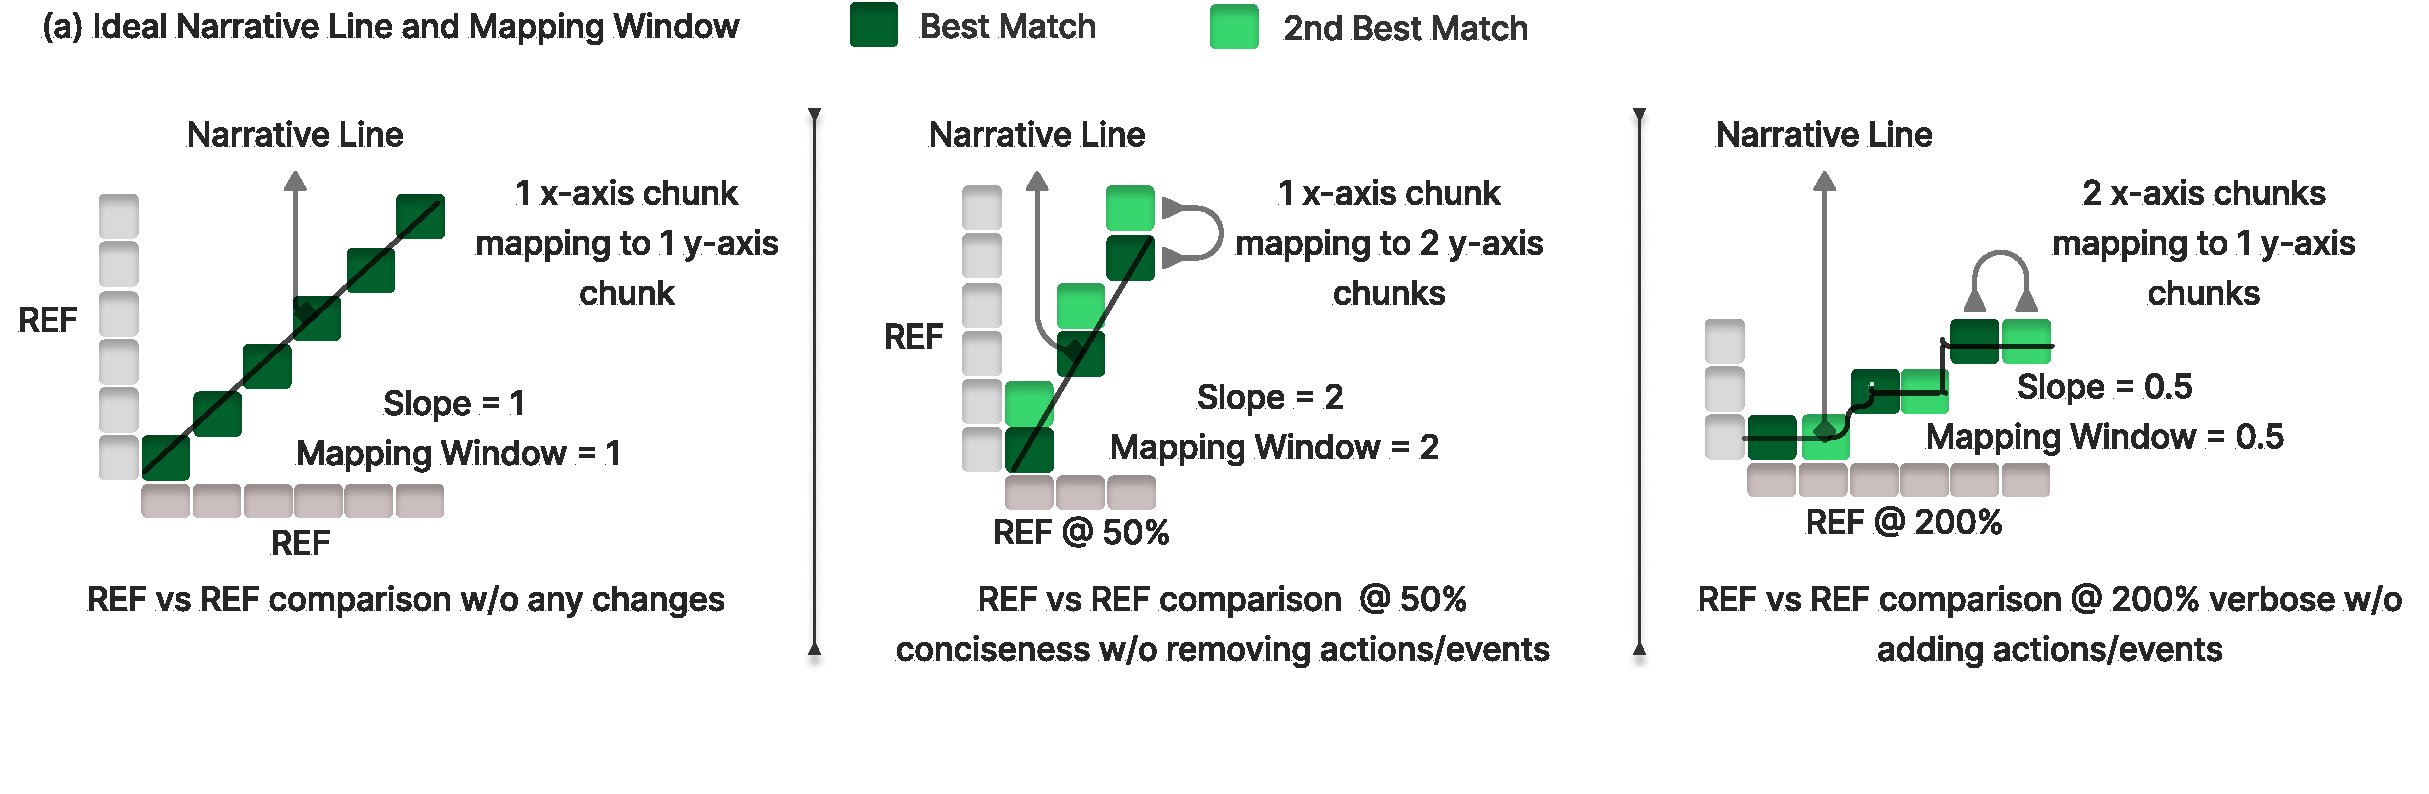
\includegraphics[width=1\textwidth]{mapping_window.pdf} % Adjust width as needed, or use other options like scale, height.
  \caption{Illustration of Mapping Windows: (a) Ideal 1-to-1, (b) Concise $\Tgen$ (e.g., 1 ref chunk to 2 gen chunks), (c) Verbose $\Tgen$ (e.g., 2 ref chunks to 1 gen chunk).}
  \label{fig:mapping_windows} % Optional: for cross-referencing the figure in your text
\end{figure}

\paragraph{Best Matching Algorithm} % Title from new text (no period)
\label{sssec:best_matching_revised} % From new text
The Best Matching Algorithm establishes robust one-to-one chunk/word correspondences, resolving semantic ambiguity and collisions inherent in naive highest-similarity pairing. For each source element, it identifies the maximum similarity ($\Mj$). If $\Mj$ exceeds a context cutoff (e.g., 0.6), an adaptive similarity margin (influenced by $\Mj$) defines a candidate band. From candidates within this band, the one closest to its expected narrative position (defined by $\MWprec$ or $\MWrec$) is selected. Ties are broken by highest raw similarity. This bidirectional process yields precision-oriented ($\MP$) and recall-oriented ($\MR$) best matches.

\subsubsection{Local Alignment Score (LAS)} % From template
\label{ssec:las_revised} % From new text
The Local Alignment Score (LAS) assesses fine-grained semantic quality, averaging cosine similarities of matched chunk/word pairs from Section~\ref{sssec:best_matching_revised}. It computes precision-oriented $\LASP = \frac{\sum_{(c_{j}^{\text{gen}},c_{m(j)}^{\text{ref}})\in \MP}\Sim(c_{j}^{\text{gen}},c_{m(j)}^{\text{ref}})}{|\MP|}$ (if $|\MP|>0$, else 0) and recall-oriented $\LASR = \frac{\sum_{(c_{i}^{\text{ref}},c_{m(i)}^{\text{gen}})\in \MR}\Sim(c_{i}^{\text{ref}},c_{m(i)}^{\text{gen}})}{|\MR|}$ (if $|\MR|>0$, else 0). The final LAS is their harmonic mean:
\begin{equation} \label{eq:las_revised}
\LAS = F_1(\LASP, \LASR) =
\begin{cases}
\frac{2 \cdot \LASP \cdot \LASR}{\LASP + \LASR} & \text{if } \LASP + \LASR > 0 \\
0 & \text{otherwise}
\end{cases}
\end{equation}
High LAS indicates strong local semantic agreement. LAS is somewhat sensitive to content gaps, though less so than NAS, and is insensitive to chronological order, motivating the Narrative Alignment Score (NAS) (Section~\ref{ssec:nas_revised}).

\subsubsection{Narrative Alignment Score (NAS)} % From template
\label{ssec:nas_revised} % From new text
The Narrative Alignment Score (NAS) evaluates narrative integrity and chronological coherence of $\Tgen$ against $\Tref$, addressing LAS's insensitivity to order and providing stronger penalties for structural discrepancies. For $\VCSshort$, NAS assesses word order.

\paragraph{Distance-based NAS ($\NASD$)} % Title from new text (no period)
\label{sssec:nasd_revised} % From new text
$\NASD$ assesses chronological alignment by penalizing deviations of matched elements ($\MP, \MR$) from expected positions within Mapping Windows (Section~\ref{sssec:mapping_window_revised}). It is largely sensitive to global misalignments (penalized more) and somewhat to local misalignments and content gaps. For each match, an effective distance $\dprime$ (incorporating LCT, Section~\ref{sssec:lct_revised}) contributes to a total penalty $\Ptotalx$. Normalizing by maximum possible penalty $\Pmaxx$ (Fig.~\ref{fig:max_penalty}) yields $\NASDP$ and $\NASDR$:
\begin{figure}[ht] % You can adjust placement options like [htbp]
  \centering
  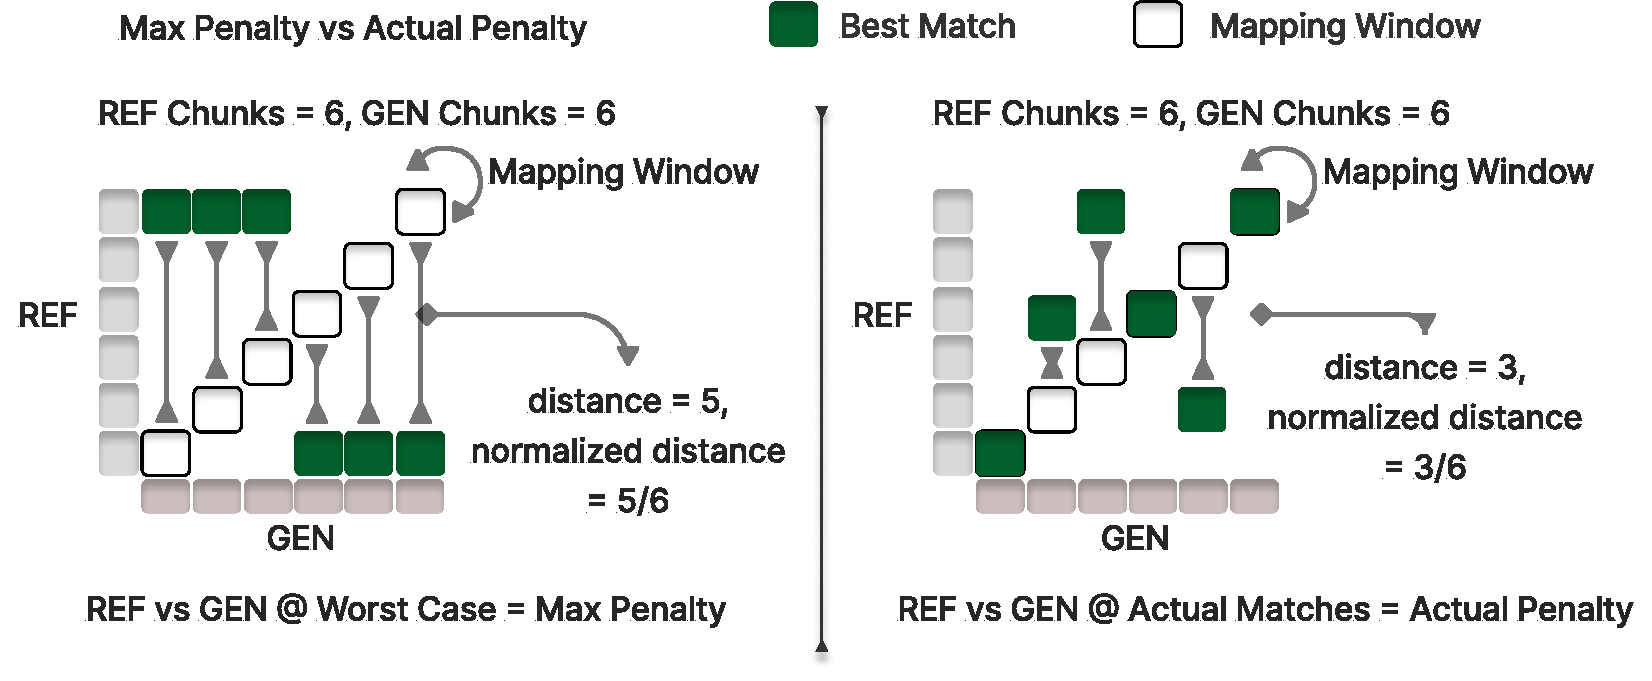
\includegraphics[width=1\textwidth]{MaxP.pdf} % Adjust width as needed, or use other options like scale, height.
  \caption{Illustration of Mapping Windows: (a) Ideal 1-to-1, (b) Concise $\Tgen$ (e.g., 1 ref chunk to 2 gen chunks), (c) Verbose $\Tgen$ (e.g., 2 ref chunks to 1 gen chunk).}
  \label{fig:max_penalty} % Optional: for cross-referencing the figure in your text
\end{figure}
\begin{equation} \label{eq:nas_dx_revised}
\text{NAS}_{Dx} =
\begin{cases}
1 - \frac{\Ptotalx}{\Pmaxx} & \text{if } \Pmaxx > 0 \\
1.0 & \text{if } \Pmaxx = 0 \text{ and } \Ptotalx = 0 \\
0.0 & \text{if } \Pmaxx = 0 \text{ and } \Ptotalx > 0
\end{cases}
\quad (x \in \{P, R\})
\end{equation}
$\NASD$ is the harmonic mean of $\NASDP$ and $\NASDR$:
\begin{equation} \label{eq:nas_d_revised}
\NASD = F_1(\NASDP, \NASDR)
\end{equation}

\paragraph{Line-based NAS ($\NASL$)} % Title from new text (no period)
\label{sssec:nasl_revised} % From new text
$\NASL$ evaluates local chronological flow by analyzing the path of consecutive matched elements. It is highly sensitive to local chronology and content gaps, and less sensitive to global misalignments compared to $\NASD$. An ideal path lies within an "ideal narrative band" (Fig.~\ref{fig:max_penalty}), bounded by estimated shortest ($\Lflooridealx$) and estimated longest ($\Lceilidealx$) path lengths. The actual path length ($\Lactualx$), from valid segment lengths (using LCT, Section~\ref{sssec:lct_revised}), is penalized for deviations:

\begin{equation} \label{eq:nas_lx_revised}
\text{NAS}_{Lx} =
\begin{cases}
1.0 & \text{if } \Lflooridealx \leq \Lactualx \leq \Lceilidealx \\
\Lactualx / \Lflooridealx & \text{if } \Lactualx < \Lflooridealx \text{ and } \Lflooridealx > 0 \\
\Lceilidealx / \Lactualx & \text{if } \Lactualx > \Lceilidealx \text{ and } \Lactualx > 0 \\
0.0 & \text{otherwise}
\end{cases}
\quad (x \in \{P, R\})
\end{equation}
$\NASL$ is the harmonic mean of $\NASLP$ and $\NASLR$:
\begin{equation} \label{eq:nas_l_revised}
\NASL = F_1(\NASLP, \NASLR)
\end{equation}

\paragraph{Local Chronology Tolerance (LCT)} % Title from new text (no period)
\label{sssec:lct_revised} % From new text
LCT (multiplier $\tauLCT \geq 0$) allows configurable flexibility for benign local reorderings and can add tolerance to minor content additions/omissions. In $\NASD$, it widens permissible deviation from Mapping Windows before penalty. In $\NASL$, it expands acceptable step variations between matches. $\tauLCT=0$ enforces strict order.

\paragraph{Final Narrative Alignment Score ($\NASFone$)} % Title from new text (no period)
\label{sssec:nas_f1_revised} % From new text
$\NASD$ (Eq.~\ref{eq:nas_d_revised}) and $\NASL$ (Eq.~\ref{eq:nas_l_revised}) are integrated via harmonic mean to produce $\NASFone$:
\begin{equation} \label{eq:nas_f1_revised}
\NASFone = F_1(\NASD, \NASL) 
\end{equation}

\paragraph{Window Regularizer for NAS} % Title from new text (no period)
\label{sssec:window_regularizer_revised} % From new text
The Window Regularizer ($\RW$) adjusts $\NASFone$ to mitigate influence from extreme text length disparities.
Let $MW_{\text{sel}}$ be $\MWrec$ if $\Nref < \Ngen$, else $MW_{\text{sel}} = \MWprec$.
Let $N_{\text{max}} = \max(\Nref, \Ngen)$.
The total mapping window area is $\Atotalmw = \sum_{(s,e) \in MW_{\text{sel}}} (e-s)$.
The timeline area is $\Atimeline = \Nref \cdot \Ngen$.
The minimum area ratio is $\Aminratio = 1/N_{\text{max}}$ (if $N_{\text{max}}>0$, else 0).
The Window Regularizer $\RW$ is calculated as:
\begin{equation}
\RW = 
\begin{cases}
\max\left(0, \min\left(1, \frac{(\Atotalmw / \Atimeline) - \Aminratio}{0.5 - \Aminratio}\right)\right) & \text{if } \Atimeline > 0 \text{ and } \Aminratio < 1 \\
0 & \text{otherwise}
\end{cases}
\end{equation}
The denominator term $(0.5 - \Aminratio)$ uses $0.5$ as a threshold because if the mapping windows cover 50\% or more of the total timeline area, the NAS score becomes significantly less meaningful due to overly relaxed chronological constraints, warranting the regularizer to approach its maximum effect.
Let $\NASinterim = \NASFone - \RW$. The regularized score $\NASreg$ is:
\begin{equation} \label{eq:nas_reg_revised}
\NASreg =
\begin{cases}
\frac{\NASinterim}{1 - \RW} & \text{if } \NASinterim > 0 \text{ and } \RW < 1 \\
0.0 & \text{otherwise}
\end{cases}
\end{equation}
This re-normalizes so $\NASreg$ can reach 1 if $\NASFone=1$ and $\RW=0$.

\subsection{Aggregating Scores for the Final Video Comprehension Score (VCS)} % From template
\label{sec:aggregating_scores_revised} % From new text
The final VCS or $\VCSshort$ integrates semantic and narrative alignment. GAS is modulated by LAS yielding the Semantic Alignment Score ($\SAS$):
\begin{equation} \label{eq:sas_revised} 
\SAS = 
\begin{cases}
\frac{\text{GAS} - (1 - \text{LAS})}{\text{LAS}} & \text{if } \text{LAS} > 0 \text{ and } (\text{GAS} - (1 - \text{LAS})) > 0 \\
0.0 & \text{otherwise}
\end{cases}
\end{equation}
The score (VCS or $\VCSshort$) synthesizes $\SAS$ with $\NASreg$ (Eq.~\ref{eq:nas_reg_revised}).
Let $S_{\text{num}}$ and $S_{\text{den}}$ be defined based on $\SAS$ and $\NASreg$:
\begin{align*}
S_{\text{num}} &= 
\begin{cases}
\SAS - (1 - \NASreg) & \text{if } \SAS < \NASreg \\
\NASreg - (1 - \SAS) & \text{otherwise}
\end{cases} \\
S_{\text{den}} &= 
\begin{cases}
\NASreg & \text{if } \SAS < \NASreg \\
\SAS & \text{otherwise}
\end{cases}
\end{align*}
The final score is:
\begin{equation} \label{eq:vcs_revised}
\text{VCS (or } \VCSshort\text{)} =
\begin{cases}
\frac{S_{\text{num}}}{S_{\text{den}}} & \text{if } S_{\text{num}} > 0 \text{ and } S_{\text{den}} \neq 0 \\
0.0 & \text{otherwise}
\end{cases}
\end{equation}

\subsection{\texorpdfstring{$\VCSshort$}{VCSshort}: Extension for Short Captions} % New section from new text
\label{sec:vcs_short} % From new text
VCS can be adapted for evaluating short captions at the word level, termed $\VCSshort$. The core metric suite (GAS, LAS, NAS) and aggregation logic (Section~\ref{sec:vcs_metric_suite_revised} and \ref{sec:aggregating_scores_revised}) remain consistent. The primary distinction lies in the initial text preprocessing.

\subsubsection{Text Preprocessing for \texorpdfstring{$\VCSshort$}{VCSshort}} % New subsection from new text
For $\VCSshort$, input texts $\Tref$ and $\Tgen$ are first cleaned by removing all punctuation and stop words. After this cleaning, the texts are tokenized into individual words. These words then serve as the fundamental "segments" or "elements" for all subsequent alignment and scoring processes, replacing the multi-word chunks used in the standard VCS. Each word is then embedded using $\nvEmbed$\cite{lee2024nv} for comparison. 
\section{Experiments}
We conduct experiments to validate Video Comprehension Score (VCS) on large-scale synthetic datasets designed specifically to evaluate robustness in assessing long-form video descriptions. Our evaluation targets three core challenges: the many-to-one mapping problem, chronological accuracy (local and global), and precise content alignment.

We construct the synthetic dataset from the MPII Movie Description (MPII-MD) dataset \cite{rohrbach2015dataset}, consisting of detailed audio descriptions temporally aligned with movie scenes. From MPII-MD's 94 movies, scene-level descriptions are aggregated into coherent narratives via ChatGPT-4o \cite{achiam2023gpt}, generating 1,390 baseline descriptions averaging 500 words each.

To test robustness, we systematically produce two types of description variants using ChatGPT-4o \cite{achiam2023gpt}:

\textbf{Valid variants (12,510 total)} include lexical/syntactic paraphrases (synonym substitutions, active/passive voice transformations), descriptive length and detail variations (brevity: \textasciitilde70\%, \textasciitilde50\%; verbosity: \textasciitilde120\%, \textasciitilde130\%), granularity transformations (macro-to-micro, micro-to-macro actions), and attribute/emotion/scene enrichments.\\
\textbf{Invalid variants} introduce deliberate errors in content alignment (redundant content, unrelated additions, content deletion, semantic corruption, complete incoherence, lossy summarization) and chronology (paragraph rotation, complete reversal, sentence shuffling, neighboring sentence swaps).


Additionally, to simulate realistic multi-author variability, we generated a "Multiple-Author Test Set" by prompting four distinct LLMs (ChatGPT-4o, Grok, Mistral, Claude) to independently rewrite each baseline scene description (yielding 5,560 descriptions). These models were instructed to preserve original narrative events and chronology but were free to introduce various valid stylistic transformations.

We benchmark VCS against established metrics, including traditional n-gram-based measures (BLEU-1/4 \cite{papineni2002bleu}, ROUGE \cite{lin2004rouge} variants and METEOR \cite{banerjee2005meteor}) and novel segment-based semantic adaptations using SaT segmentation \cite{frohmann2024segment} and nv-embed-v2 \cite{lee2024nv} embeddings (Segment-BLEU, Segment-METEOR, Segment-ROUGE-L). Segment matching was established via cosine similarity thresholding (0.75).

For shorter descriptions, we evaluated VCS\textsubscript{short} on VATEX-EVAL \cite{shi2022emscore}, correlating metric scores with human judgments (Kendall's $\tau_b$, Spearman's $\rho$) under single and multiple reference scenarios. We compared VCS\textsubscript{short} to standard n-gram metrics (BLEU \cite{papineni2002bleu}, ROUGE \cite{lin2004rouge}, METEOR \cite{banerjee2005meteor}, CIDEr \cite{vedantam2015cider}) and embedding-based metrics (BERTScore \cite{zhang2019bertscore}, BERTScore++ \cite{yi2020improving}), alongside multimodal embedding metrics (EMScore \cite{shi2022emscore}, PAC-S/RefPAC-S \cite{sarto2023positive}).
\section{Results}

\begin{table}
  \caption{Performance comparison of different metrics on various test cases. For each metric, the top value represents the average and the bottom value represents the standard deviation.}
  \label{tab:mpii-aug-eval}
  \centering
  \setlength{\tabcolsep}{3pt}
  \begin{adjustbox}{max width=\textwidth}
    \begin{tabular}{@{}cc@{\hskip 2pt}p{2.2cm}*{9}{c}@{\hskip 15pt}*{11}{c}@{}}
      \toprule
      & & & 
      \rotatebox{80}{\textbf{Synonym Substitution}} &
      \rotatebox{80}{\textbf{Active $\leftrightarrow$ Passive}} &
      \rotatebox{80}{\textbf{Brevity - L1}} &
      \rotatebox{80}{\textbf{Brevity - L2}} &
      \rotatebox{80}{\textbf{Verbosity - L1}} &
      \rotatebox{80}{\textbf{Verbosity - L2}} &
      \rotatebox{80}{\textbf{Macro $\rightarrow$ Micro}} &
      \rotatebox{80}{\textbf{Micro $\rightarrow$ Macro}} &
      \rotatebox{80}{\textbf{Insert Attr./Emotions}} &
      \rotatebox{80}{\textbf{Scattered Repetition}} &
      \rotatebox{80}{\textbf{Addition (50\%)}} &
      \rotatebox{80}{\textbf{Addition (80\%)}} &
      \rotatebox{80}{\textbf{Deletion (50\%)}} &
      \rotatebox{80}{\textbf{Deletion (80\%)}} &
      \rotatebox{80}{\textbf{Subject-Action-Obj}} &
      \rotatebox{80}{\textbf{Complete Corruption}} &
      \rotatebox{80}{\textbf{Summarization}} &
      \rotatebox{80}{\textbf{Reverse Segments}} &
      \rotatebox{80}{\textbf{Jumble Segments}} &
      \rotatebox{80}{\textbf{Rotate Half Para}} \\
      \cmidrule(lr{15pt}){4-12} \cmidrule{13-23}
      
      & & \textbf{Metric} & 
      \multicolumn{9}{c}{\textbf{Valid Test Cases}} & 
      \multicolumn{11}{c}{\textbf{Invalid Test Cases}} \\
      \midrule
      
      \multirow{14}{*}{\rotatebox[origin=cB]{90}{\textbf{Traditional}}} & & BLEU-1 \cite{papineni2002bleu} & 0.831 & 0.798 & 0.383 & 0.234 & 0.665 & 0.557 & 0.573 & 0.340 & 0.695 & 0.661 & 0.540 & 0.437 & 0.389 & 0.037 & 0.494 & 0.321 & 0.081 & 0.997 & 0.997 & 0.997 \\
      & & & 0.085 & 0.057 & 0.144 & 0.118 & 0.089 & 0.072 & 0.089 & 0.129 & 0.065 & 0.021 & 0.069 & 0.070 & 0.070 & 0.028 & 0.046 & 0.029 & 0.054 & 0.005 & 0.005 & 0.005 \\
      \cmidrule(lr{15pt}){4-12} \cmidrule{13-23}
      
      & & BLEU-4 \cite{papineni2002bleu} & 0.631 & 0.528 & 0.186 & 0.094 & 0.366 & 0.255 & 0.252 & 0.131 & 0.625 & 0.647 & 0.535 & 0.433 & 0.385 & 0.036 & 0.105 & 0.007 & 0.022 & 0.902 & 0.904 & 0.992 \\
      & & & 0.157 & 0.108 & 0.115 & 0.071 & 0.144 & 0.092 & 0.108 & 0.084 & 0.084 & 0.025 & 0.069 & 0.070 & 0.070 & 0.027 & 0.046 & 0.003 & 0.021 & 0.036 & 0.037 & 0.010 \\
      \cmidrule(lr{15pt}){4-12} \cmidrule{13-23}
      
      & & METEOR \cite{banerjee2005meteor} & 0.880 & 0.870 & 0.393 & 0.295 & 0.698 & 0.632 & 0.587 & 0.335 & 0.864 & 0.768 & 0.826 & 0.794 & 0.472 & 0.210 & 0.501 & 0.232 & 0.176 & 0.589 & 0.644 & 0.632 \\
      & & & 0.071 & 0.053 & 0.111 & 0.083 & 0.112 & 0.087 & 0.089 & 0.091 & 0.044 & 0.070 & 0.024 & 0.029 & 0.045 & 0.038 & 0.063 & 0.015 & 0.045 & 0.032 & 0.034 & 0.037 \\
      \cmidrule(lr{15pt}){4-12} \cmidrule{13-23}
      
      & & ROUGE-1 \cite{lin2004rouge} & 0.839 & 0.897 & 0.640 & 0.541 & 0.774 & 0.700 & 0.695 & 0.581 & 0.818 & 0.791 & 0.697 & 0.605 & 0.670 & 0.360 & 0.514 & 0.346 & 0.372 & 0.990 & 0.990 & 0.990 \\
      & & & 0.081 & 0.031 & 0.096 & 0.093 & 0.068 & 0.060 & 0.071 & 0.093 & 0.046 & 0.016 & 0.060 & 0.070 & 0.043 & 0.053 & 0.045 & 0.027 & 0.070 & 0.009 & 0.009 & 0.009 \\
      \cmidrule(lr{15pt}){4-12} \cmidrule{13-23}
      
      & & ROUGE-4 \cite{lin2004rouge} & 0.502 & 0.411 & 0.157 & 0.089 & 0.257 & 0.164 & 0.154 & 0.095 & 0.663 & 0.743 & 0.674 & 0.584 & 0.642 & 0.335 & 0.025 & 0.000 & 0.029 & 0.792 & 0.796 & 0.962 \\
      & & & 0.189 & 0.126 & 0.102 & 0.062 & 0.152 & 0.090 & 0.101 & 0.068 & 0.093 & 0.037 & 0.061 & 0.070 & 0.047 & 0.055 & 0.021 & 0.000 & 0.023 & 0.066 & 0.067 & 0.027 \\
      \cmidrule(lr{15pt}){4-12} \cmidrule{13-23}
      
      & & ROUGE-L \cite{lin2004rouge} & 0.834 & 0.754 & 0.556 & 0.456 & 0.698 & 0.606 & 0.577 & 0.452 & 0.816 & 0.789 & 0.696 & 0.603 & 0.669 & 0.360 & 0.472 & 0.153 & 0.274 & 0.231 & 0.365 & 0.535 \\
      & & & 0.084 & 0.065 & 0.112 & 0.098 & 0.100 & 0.084 & 0.097 & 0.100 & 0.047 & 0.016 & 0.060 & 0.070 & 0.043 & 0.053 & 0.055 & 0.010 & 0.065 & 0.023 & 0.046 & 0.032 \\
      \cmidrule(lr{15pt}){4-12} \cmidrule{13-23}
      
      & & ROUGE-Lsum \cite{lin2004rouge} & 0.838 & 0.848 & 0.621 & 0.521 & 0.761 & 0.684 & 0.676 & 0.554 & 0.818 & 0.790 & 0.697 & 0.604 & 0.670 & 0.360 & 0.507 & 0.335 & 0.352 & 0.967 & 0.977 & 0.988 \\
      & & & 0.082 & 0.041 & 0.100 & 0.094 & 0.073 & 0.063 & 0.074 & 0.094 & 0.046 & 0.016 & 0.060 & 0.070 & 0.043 & 0.053 & 0.045 & 0.026 & 0.068 & 0.024 & 0.019 & 0.011 \\
      \midrule
      
      \multirow{12}{*}{\rotatebox[origin=cB]{90}{\textbf{Ablation}}} & & GAS & 0.948 & 0.978 & 0.950 & 0.928 & 0.951 & 0.915 & 0.933 & 0.929 & 0.888 & 0.922 & 0.803 & 0.732 & 0.900 & 0.764 & 0.525 & 0.184 & 0.871 & 0.954 & 0.955 & 0.955 \\
      & & & 0.064 & 0.016 & 0.023 & 0.026 & 0.029 & 0.035 & 0.035 & 0.030 & 0.036 & 0.026 & 0.054 & 0.096 & 0.034 & 0.060 & 0.072 & 0.054 & 0.042 & 0.012 & 0.014 & 0.013 \\
      \cmidrule(lr{15pt}){4-12} \cmidrule{13-23}
      
      & & LAS & 0.911 & 0.906 & 0.765 & 0.709 & 0.855 & 0.814 & 0.797 & 0.694 & 0.875 & 0.986 & 0.844 & 0.798 & 0.818 & 0.653 & 0.445 & 0.237 & 0.601 & 0.977 & 0.978 & 0.978 \\
      & & & 0.056 & 0.038 & 0.070 & 0.061 & 0.053 & 0.049 & 0.055 & 0.072 & 0.034 & 0.014 & 0.020 & 0.021 & 0.026 & 0.044 & 0.069 & 0.029 & 0.062 & 0.019 & 0.019 & 0.019 \\
      \cmidrule(lr{15pt}){4-12} \cmidrule{13-23}
      
      & & NAS & 0.981 & 0.958 & 0.878 & 0.832 & 0.948 & 0.929 & 0.921 & 0.846 & 0.961 & 0.736 & 0.794 & 0.737 & 0.670 & 0.234 & 0.862 & 0.210 & 0.734 & 0.007 & 0.064 & 0.455 \\
      & & & 0.052 & 0.039 & 0.083 & 0.092 & 0.043 & 0.049 & 0.053 & 0.092 & 0.038 & 0.055 & 0.029 & 0.032 & 0.037 & 0.115 & 0.128 & 0.077 & 0.132 & 0.019 & 0.055 & 0.026 \\
      \cmidrule(lr{15pt}){4-12} \cmidrule{13-23}
      
      & & GAS+LAS & 0.942 & 0.976 & 0.932 & 0.895 & 0.941 & 0.894 & 0.914 & 0.894 & 0.871 & 0.921 & 0.767 & 0.665 & 0.877 & 0.635 & 0.070 & 0.000 & 0.779 & 0.953 & 0.954 & 0.954 \\
      & & & 0.070 & 0.018 & 0.036 & 0.044 & 0.037 & 0.047 & 0.048 & 0.053 & 0.043 & 0.026 & 0.063 & 0.117 & 0.044 & 0.108 & 0.115 & 0.000 & 0.092 & 0.013 & 0.014 & 0.014 \\
      \cmidrule(lr{15pt}){4-12} \cmidrule{13-23}

      & & NAS+LAS & 0.909 & 0.899 & 0.724 & 0.639 & 0.844 & 0.797 & 0.776 & 0.626 & 0.869 & 0.732 & 0.755 & 0.669 & 0.596 & 0.011 & 0.345 & 0.000 & 0.433 & 0.003 & 0.049 & 0.442 \\ 
      & & & 0.061 & 0.045 & 0.105 & 0.111 & 0.061 & 0.060 & 0.069 & 0.124 & 0.039 & 0.057 & 0.038 & 0.045 & 0.052 & 0.032 & 0.155 & 0.000 & 0.168 & 0.009 & 0.050 & 0.033 \\
      \cmidrule(lr{15pt}){4-12} \cmidrule{13-23}
      
      & & GAS+LAS+NAS & 0.937 & 0.951 & 0.860 & 0.801 & 0.922 & 0.875 & 0.885 & 0.812 & 0.864 & 0.714 & 0.691 & 0.534 & 0.622 & 0.019 & 0.050 & 0.000 & 0.623 & 0.001 & 0.034 & 0.428 \\
      & & & 0.072 & 0.037 & 0.088 & 0.101 & 0.046 & 0.054 & 0.059 & 0.105 & 0.047 & 0.057 & 0.068 & 0.141 & 0.049 & 0.049 & 0.102 & 0.000 & 0.182 & 0.008 & 0.044 & 0.028 \\
      \bottomrule
    \end{tabular}
  \end{adjustbox}
\end{table}

\begin{table}
  \caption{Human judgment correlation scores on VATEX-EVAL dataset \cite{shi2022emscore}.}
  \label{tab:vatex-eval}
  \centering
  \begin{tabular}{lcccc}
    \toprule
    & \multicolumn{2}{c}{\textbf{1Ref}} & \multicolumn{2}{c}{\textbf{9Refs}} \\
    \cmidrule(r){2-3} \cmidrule(r){4-5}
    & Kendall $\tau_b$ & Spearman $\rho$ & Kendall $\tau_b$ & Spearman $\rho$ \\
    \midrule
    BLEU-1 \cite{papineni2002bleu} & 12.2 & 15.9 & 28.9 & 37.0 \\
    BLEU-4 \cite{papineni2002bleu} & 12.6 & 16.4 & 22.4 & 29.5 \\
    ROUGE \cite{lin2004rouge} & 12.5 & 16.3 & 23.8 & 30.9 \\
    METEOR \cite{banerjee2005meteor} & 16.4 & 21.5 & 27.6 & 35.7 \\
    CIDEr \cite{vedantam2015cider} & 17.3 & 22.6 & 27.8 & 36.1 \\
    \midrule
    BERT-S \cite{zhang2019bertscore} & 18.2 & 23.7 & 29.3 & 37.8 \\
    BERT-S++ \cite{yi2020improving} & 15.2 & 19.8 & 24.4 & 31.7 \\
    \midrule
    EMScore \cite{shi2022emscore} & 28.6 & 37.1 & 36.8 & 47.2 \\
    PAC-S / RefPAC-S \cite{sarto2023positive} & \cellcolor{green!20}31.4 & \cellcolor{green!20}40.5 & \cellcolor{orange!25}38.1 & \cellcolor{orange!25}48.8 \\
    \midrule
    VCS & \cellcolor{orange!25}30.0 & \cellcolor{orange!25}38.1 & \cellcolor{green!20}41.5 & \cellcolor{green!20}52.8 \\
    \bottomrule
  \end{tabular}
\end{table}

\begin{table}[htbp]
  \caption{Performance comparison of different metrics across various authorial combinations. For each metric, the top value represents the average and the bottom value represents the standard deviation.}
  \label{tab:mpii-authors}
  \centering
  \setlength{\tabcolsep}{5.6pt} % Adjust inter-column spacing if needed
  \begin{adjustbox}{max width=\textwidth}
    \begin{tabular}{@{}l*{12}{c}@{}}
      \toprule
      \textbf{Metric} & \multicolumn{3}{c}{\textbf{Author 1}} & \multicolumn{3}{c}{\textbf{Author 2}} & \multicolumn{3}{c}{\textbf{Author 3}} & \multicolumn{3}{c}{\textbf{Author 4}} \\
      \cmidrule(lr){2-4} \cmidrule(lr){5-7} \cmidrule(lr){8-10} \cmidrule(lr){11-13}
                      & A1-A2 & A1-A3 & A1-A4 & A2-A1 & A2-A3 & A2-A4 & A3-A1 & A3-A2 & A3-A4 & A4-A1 & A4-A2 & A4-A3 \\
      \midrule
      BLEU-1 \cite{papineni2002bleu}        & 0.476 & 0.818 & 0.777 & 0.495 & 0.494 & 0.511 & 0.816 & 0.473 & 0.813 & 0.781 & 0.497 & 0.820 \\
                    & 0.077 & 0.144 & 0.185 & 0.066 & 0.064 & 0.066 & 0.147 & 0.076 & 0.193 & 0.178 & 0.076 & 0.184 \\
      \cmidrule(lr){2-13}
      BLEU-4 \cite{papineni2002bleu}        & 0.126 & 0.592 & 0.555 & 0.130 & 0.133 & 0.140 & 0.591 & 0.128 & 0.639 & 0.557 & 0.136 & 0.641 \\
                    & 0.045 & 0.284 & 0.299 & 0.044 & 0.045 & 0.046 & 0.285 & 0.045 & 0.341 & 0.297 & 0.047 & 0.339 \\
      \cmidrule(lr){2-13}
      METEOR \cite{banerjee2005meteor}        & 0.379 & 0.741 & 0.705 & 0.456 & 0.456 & 0.455 & 0.725 & 0.368 & 0.754 & 0.716 & 0.388 & 0.782 \\
                    & 0.058 & 0.174 & 0.210 & 0.045 & 0.049 & 0.048 & 0.186 & 0.053 & 0.234 & 0.199 & 0.062 & 0.210 \\
      \cmidrule(lr){2-13}
      ROUGE-1 \cite{lin2004rouge}       & 0.601 & 0.862 & 0.838 & 0.601 & 0.606 & 0.613 & 0.862 & 0.606 & 0.868 & 0.838 & 0.613 & 0.868 \\
                    & 0.054 & 0.115 & 0.140 & 0.054 & 0.055 & 0.053 & 0.115 & 0.055 & 0.138 & 0.140 & 0.053 & 0.138 \\
      \cmidrule(lr){2-13}
      ROUGE-4 \cite{lin2004rouge}       & 0.051 & 0.502 & 0.475 & 0.051 & 0.055 & 0.057 & 0.502 & 0.055 & 0.583 & 0.475 & 0.057 & 0.583 \\
                    & 0.027 & 0.323 & 0.322 & 0.027 & 0.029 & 0.029 & 0.323 & 0.029 & 0.381 & 0.322 & 0.029 & 0.381 \\
      \cmidrule(lr){2-13}
      ROUGE-L \cite{lin2004rouge}       & 0.414 & 0.786 & 0.753 & 0.414 & 0.416 & 0.421 & 0.786 & 0.416 & 0.785 & 0.753 & 0.421 & 0.785 \\
                    & 0.059 & 0.183 & 0.210 & 0.059 & 0.058 & 0.057 & 0.183 & 0.058 & 0.225 & 0.210 & 0.057 & 0.225 \\
      \cmidrule(lr){2-13}
      ROUGE-Lsum \cite{lin2004rouge}    & 0.566 & 0.849 & 0.824 & 0.566 & 0.574 & 0.580 & 0.850 & 0.575 & 0.855 & 0.825 & 0.581 & 0.855 \\

      \cmidrule(lr){2-13}
      VCS   & 0.857 & 0.933 & 0.916 & 0.857 & 0.843 & 0.850 & 0.933 & 0.843 & 0.934 & 0.916 & 0.850 & 0.934 \\
                    & 0.108 & 0.078 & 0.109 & 0.108 & 0.117 & 0.112 & 0.078 & 0.117 & 0.099 & 0.109 & 0.112 & 0.099 \\
      \bottomrule
    \end{tabular}
  \end{adjustbox}
\end{table}




\begin{ack}
Use unnumbered first level headings for the acknowledgments. All acknowledgments
go at the end of the paper before the list of references. Moreover, you are required to declare
funding (financial activities supporting the submitted work) and competing interests (related financial activities outside the submitted work).
More information about this disclosure can be found at: \url{https://neurips.cc/Conferences/2025/PaperInformation/FundingDisclosure}.


Do {\bf not} include this section in the anonymized submission, only in the final paper. You can use the \texttt{ack} environment provided in the style file to automatically hide this section in the anonymized submission.
\end{ack}

\FloatBarrier
%\section*{References}
\medskip 

{
\small % Reduce font size as permissible

\bibliographystyle{unsrtnat}
\bibliography{references}

} % End the group for \small


%%%%%%%%%%%%%%%%%%%%%%%%%%%%%%%%%%%%%%%%%%%%%%%%%%%%%%%%%%%%

\appendix

\section{Technical Appendices and Supplementary Material}
Technical appendices with additional results, figures, graphs and proofs may be submitted with the paper submission before the full submission deadline (see above), or as a separate PDF in the ZIP file below before the supplementary material deadline. There is no page limit for the technical appendices.

%%%%%%%%%%%%%%%%%%%%%%%%%%%%%%%%%%%%%%%%%%%%%%%%%%%%%%%%%%%%

\newpage
\section*{NeurIPS Paper Checklist}

%%% BEGIN INSTRUCTIONS %%%
The checklist is designed to encourage best practices for responsible machine learning research, addressing issues of reproducibility, transparency, research ethics, and societal impact. Do not remove the checklist: {\bf The papers not including the checklist will be desk rejected.} The checklist should follow the references and follow the (optional) supplemental material.  The checklist does NOT count towards the page
limit. 

Please read the checklist guidelines carefully for information on how to answer these questions. For each question in the checklist:
\begin{itemize}
    \item You should answer \answerYes{}, \answerNo{}, or \answerNA{}.
    \item \answerNA{} means either that the question is Not Applicable for that particular paper or the relevant information is Not Available.
    \item Please provide a short (1–2 sentence) justification right after your answer (even for NA). 
   % \item {\bf The papers not including the checklist will be desk rejected.}
\end{itemize}

{\bf The checklist answers are an integral part of your paper submission.} They are visible to the reviewers, area chairs, senior area chairs, and ethics reviewers. You will be asked to also include it (after eventual revisions) with the final version of your paper, and its final version will be published with the paper.

The reviewers of your paper will be asked to use the checklist as one of the factors in their evaluation. While "\answerYes{}" is generally preferable to "\answerNo{}", it is perfectly acceptable to answer "\answerNo{}" provided a proper justification is given (e.g., "error bars are not reported because it would be too computationally expensive" or "we were unable to find the license for the dataset we used"). In general, answering "\answerNo{}" or "\answerNA{}" is not grounds for rejection. While the questions are phrased in a binary way, we acknowledge that the true answer is often more nuanced, so please just use your best judgment and write a justification to elaborate. All supporting evidence can appear either in the main paper or the supplemental material, provided in appendix. If you answer \answerYes{} to a question, in the justification please point to the section(s) where related material for the question can be found.

IMPORTANT, please:
\begin{itemize}
    \item {\bf Delete this instruction block, but keep the section heading ``NeurIPS Paper Checklist"},
    \item  {\bf Keep the checklist subsection headings, questions/answers and guidelines below.}
    \item {\bf Do not modify the questions and only use the provided macros for your answers}.
\end{itemize} 
 

%%% END INSTRUCTIONS %%%


\begin{enumerate}

\item {\bf Claims}
    \item[] Question: Do the main claims made in the abstract and introduction accurately reflect the paper's contributions and scope?
    \item[] Answer: \answerTODO{} % Replace by \answerYes{}, \answerNo{}, or \answerNA{}.
    \item[] Justification: \justificationTODO{}
    \item[] Guidelines:
    \begin{itemize}
        \item The answer NA means that the abstract and introduction do not include the claims made in the paper.
        \item The abstract and/or introduction should clearly state the claims made, including the contributions made in the paper and important assumptions and limitations. A No or NA answer to this question will not be perceived well by the reviewers. 
        \item The claims made should match theoretical and experimental results, and reflect how much the results can be expected to generalize to other settings. 
        \item It is fine to include aspirational goals as motivation as long as it is clear that these goals are not attained by the paper. 
    \end{itemize}

\item {\bf Limitations}
    \item[] Question: Does the paper discuss the limitations of the work performed by the authors?
    \item[] Answer: \answerTODO{} % Replace by \answerYes{}, \answerNo{}, or \answerNA{}.
    \item[] Justification: \justificationTODO{}
    \item[] Guidelines:
    \begin{itemize}
        \item The answer NA means that the paper has no limitation while the answer No means that the paper has limitations, but those are not discussed in the paper. 
        \item The authors are encouraged to create a separate "Limitations" section in their paper.
        \item The paper should point out any strong assumptions and how robust the results are to violations of these assumptions (e.g., independence assumptions, noiseless settings, model well-specification, asymptotic approximations only holding locally). The authors should reflect on how these assumptions might be violated in practice and what the implications would be.
        \item The authors should reflect on the scope of the claims made, e.g., if the approach was only tested on a few datasets or with a few runs. In general, empirical results often depend on implicit assumptions, which should be articulated.
        \item The authors should reflect on the factors that influence the performance of the approach. For example, a facial recognition algorithm may perform poorly when image resolution is low or images are taken in low lighting. Or a speech-to-text system might not be used reliably to provide closed captions for online lectures because it fails to handle technical jargon.
        \item The authors should discuss the computational efficiency of the proposed algorithms and how they scale with dataset size.
        \item If applicable, the authors should discuss possible limitations of their approach to address problems of privacy and fairness.
        \item While the authors might fear that complete honesty about limitations might be used by reviewers as grounds for rejection, a worse outcome might be that reviewers discover limitations that aren't acknowledged in the paper. The authors should use their best judgment and recognize that individual actions in favor of transparency play an important role in developing norms that preserve the integrity of the community. Reviewers will be specifically instructed to not penalize honesty concerning limitations.
    \end{itemize}

\item {\bf Theory assumptions and proofs}
    \item[] Question: For each theoretical result, does the paper provide the full set of assumptions and a complete (and correct) proof?
    \item[] Answer: \answerTODO{} % Replace by \answerYes{}, \answerNo{}, or \answerNA{}.
    \item[] Justification: \justificationTODO{}
    \item[] Guidelines:
    \begin{itemize}
        \item The answer NA means that the paper does not include theoretical results. 
        \item All the theorems, formulas, and proofs in the paper should be numbered and cross-referenced.
        \item All assumptions should be clearly stated or referenced in the statement of any theorems.
        \item The proofs can either appear in the main paper or the supplemental material, but if they appear in the supplemental material, the authors are encouraged to provide a short proof sketch to provide intuition. 
        \item Inversely, any informal proof provided in the core of the paper should be complemented by formal proofs provided in appendix or supplemental material.
        \item Theorems and Lemmas that the proof relies upon should be properly referenced. 
    \end{itemize}

    \item {\bf Experimental result reproducibility}
    \item[] Question: Does the paper fully disclose all the information needed to reproduce the main experimental results of the paper to the extent that it affects the main claims and/or conclusions of the paper (regardless of whether the code and data are provided or not)?
    \item[] Answer: \answerTODO{} % Replace by \answerYes{}, \answerNo{}, or \answerNA{}.
    \item[] Justification: \justificationTODO{}
    \item[] Guidelines:
    \begin{itemize}
        \item The answer NA means that the paper does not include experiments.
        \item If the paper includes experiments, a No answer to this question will not be perceived well by the reviewers: Making the paper reproducible is important, regardless of whether the code and data are provided or not.
        \item If the contribution is a dataset and/or model, the authors should describe the steps taken to make their results reproducible or verifiable. 
        \item Depending on the contribution, reproducibility can be accomplished in various ways. For example, if the contribution is a novel architecture, describing the architecture fully might suffice, or if the contribution is a specific model and empirical evaluation, it may be necessary to either make it possible for others to replicate the model with the same dataset, or provide access to the model. In general. releasing code and data is often one good way to accomplish this, but reproducibility can also be provided via detailed instructions for how to replicate the results, access to a hosted model (e.g., in the case of a large language model), releasing of a model checkpoint, or other means that are appropriate to the research performed.
        \item While NeurIPS does not require releasing code, the conference does require all submissions to provide some reasonable avenue for reproducibility, which may depend on the nature of the contribution. For example
        \begin{enumerate}
            \item If the contribution is primarily a new algorithm, the paper should make it clear how to reproduce that algorithm.
            \item If the contribution is primarily a new model architecture, the paper should describe the architecture clearly and fully.
            \item If the contribution is a new model (e.g., a large language model), then there should either be a way to access this model for reproducing the results or a way to reproduce the model (e.g., with an open-source dataset or instructions for how to construct the dataset).
            \item We recognize that reproducibility may be tricky in some cases, in which case authors are welcome to describe the particular way they provide for reproducibility. In the case of closed-source models, it may be that access to the model is limited in some way (e.g., to registered users), but it should be possible for other researchers to have some path to reproducing or verifying the results.
        \end{enumerate}
    \end{itemize}


\item {\bf Open access to data and code}
    \item[] Question: Does the paper provide open access to the data and code, with sufficient instructions to faithfully reproduce the main experimental results, as described in supplemental material?
    \item[] Answer: \answerTODO{} % Replace by \answerYes{}, \answerNo{}, or \answerNA{}.
    \item[] Justification: \justificationTODO{}
    \item[] Guidelines:
    \begin{itemize}
        \item The answer NA means that paper does not include experiments requiring code.
        \item Please see the NeurIPS code and data submission guidelines (\url{https://nips.cc/public/guides/CodeSubmissionPolicy}) for more details.
        \item While we encourage the release of code and data, we understand that this might not be possible, so “No” is an acceptable answer. Papers cannot be rejected simply for not including code, unless this is central to the contribution (e.g., for a new open-source benchmark).
        \item The instructions should contain the exact command and environment needed to run to reproduce the results. See the NeurIPS code and data submission guidelines (\url{https://nips.cc/public/guides/CodeSubmissionPolicy}) for more details.
        \item The authors should provide instructions on data access and preparation, including how to access the raw data, preprocessed data, intermediate data, and generated data, etc.
        \item The authors should provide scripts to reproduce all experimental results for the new proposed method and baselines. If only a subset of experiments are reproducible, they should state which ones are omitted from the script and why.
        \item At submission time, to preserve anonymity, the authors should release anonymized versions (if applicable).
        \item Providing as much information as possible in supplemental material (appended to the paper) is recommended, but including URLs to data and code is permitted.
    \end{itemize}


\item {\bf Experimental setting/details}
    \item[] Question: Does the paper specify all the training and test details (e.g., data splits, hyperparameters, how they were chosen, type of optimizer, etc.) necessary to understand the results?
    \item[] Answer: \answerTODO{} % Replace by \answerYes{}, \answerNo{}, or \answerNA{}.
    \item[] Justification: \justificationTODO{}
    \item[] Guidelines:
    \begin{itemize}
        \item The answer NA means that the paper does not include experiments.
        \item The experimental setting should be presented in the core of the paper to a level of detail that is necessary to appreciate the results and make sense of them.
        \item The full details can be provided either with the code, in appendix, or as supplemental material.
    \end{itemize}

\item {\bf Experiment statistical significance}
    \item[] Question: Does the paper report error bars suitably and correctly defined or other appropriate information about the statistical significance of the experiments?
    \item[] Answer: \answerTODO{} % Replace by \answerYes{}, \answerNo{}, or \answerNA{}.
    \item[] Justification: \justificationTODO{}
    \item[] Guidelines:
    \begin{itemize}
        \item The answer NA means that the paper does not include experiments.
        \item The authors should answer "Yes" if the results are accompanied by error bars, confidence intervals, or statistical significance tests, at least for the experiments that support the main claims of the paper.
        \item The factors of variability that the error bars are capturing should be clearly stated (for example, train/test split, initialization, random drawing of some parameter, or overall run with given experimental conditions).
        \item The method for calculating the error bars should be explained (closed form formula, call to a library function, bootstrap, etc.)
        \item The assumptions made should be given (e.g., Normally distributed errors).
        \item It should be clear whether the error bar is the standard deviation or the standard error of the mean.
        \item It is OK to report 1-sigma error bars, but one should state it. The authors should preferably report a 2-sigma error bar than state that they have a 96\% CI, if the hypothesis of Normality of errors is not verified.
        \item For asymmetric distributions, the authors should be careful not to show in tables or figures symmetric error bars that would yield results that are out of range (e.g. negative error rates).
        \item If error bars are reported in tables or plots, The authors should explain in the text how they were calculated and reference the corresponding figures or tables in the text.
    \end{itemize}

\item {\bf Experiments compute resources}
    \item[] Question: For each experiment, does the paper provide sufficient information on the computer resources (type of compute workers, memory, time of execution) needed to reproduce the experiments?
    \item[] Answer: \answerTODO{} % Replace by \answerYes{}, \answerNo{}, or \answerNA{}.
    \item[] Justification: \justificationTODO{}
    \item[] Guidelines:
    \begin{itemize}
        \item The answer NA means that the paper does not include experiments.
        \item The paper should indicate the type of compute workers CPU or GPU, internal cluster, or cloud provider, including relevant memory and storage.
        \item The paper should provide the amount of compute required for each of the individual experimental runs as well as estimate the total compute. 
        \item The paper should disclose whether the full research project required more compute than the experiments reported in the paper (e.g., preliminary or failed experiments that didn't make it into the paper). 
    \end{itemize}
    
\item {\bf Code of ethics}
    \item[] Question: Does the research conducted in the paper conform, in every respect, with the NeurIPS Code of Ethics \url{https://neurips.cc/public/EthicsGuidelines}?
    \item[] Answer: \answerTODO{} % Replace by \answerYes{}, \answerNo{}, or \answerNA{}.
    \item[] Justification: \justificationTODO{}
    \item[] Guidelines:
    \begin{itemize}
        \item The answer NA means that the authors have not reviewed the NeurIPS Code of Ethics.
        \item If the authors answer No, they should explain the special circumstances that require a deviation from the Code of Ethics.
        \item The authors should make sure to preserve anonymity (e.g., if there is a special consideration due to laws or regulations in their jurisdiction).
    \end{itemize}


\item {\bf Broader impacts}
    \item[] Question: Does the paper discuss both potential positive societal impacts and negative societal impacts of the work performed?
    \item[] Answer: \answerTODO{} % Replace by \answerYes{}, \answerNo{}, or \answerNA{}.
    \item[] Justification: \justificationTODO{}
    \item[] Guidelines:
    \begin{itemize}
        \item The answer NA means that there is no societal impact of the work performed.
        \item If the authors answer NA or No, they should explain why their work has no societal impact or why the paper does not address societal impact.
        \item Examples of negative societal impacts include potential malicious or unintended uses (e.g., disinformation, generating fake profiles, surveillance), fairness considerations (e.g., deployment of technologies that could make decisions that unfairly impact specific groups), privacy considerations, and security considerations.
        \item The conference expects that many papers will be foundational research and not tied to particular applications, let alone deployments. However, if there is a direct path to any negative applications, the authors should point it out. For example, it is legitimate to point out that an improvement in the quality of generative models could be used to generate deepfakes for disinformation. On the other hand, it is not needed to point out that a generic algorithm for optimizing neural networks could enable people to train models that generate Deepfakes faster.
        \item The authors should consider possible harms that could arise when the technology is being used as intended and functioning correctly, harms that could arise when the technology is being used as intended but gives incorrect results, and harms following from (intentional or unintentional) misuse of the technology.
        \item If there are negative societal impacts, the authors could also discuss possible mitigation strategies (e.g., gated release of models, providing defenses in addition to attacks, mechanisms for monitoring misuse, mechanisms to monitor how a system learns from feedback over time, improving the efficiency and accessibility of ML).
    \end{itemize}
    
\item {\bf Safeguards}
    \item[] Question: Does the paper describe safeguards that have been put in place for responsible release of data or models that have a high risk for misuse (e.g., pretrained language models, image generators, or scraped datasets)?
    \item[] Answer: \answerTODO{} % Replace by \answerYes{}, \answerNo{}, or \answerNA{}.
    \item[] Justification: \justificationTODO{}
    \item[] Guidelines:
    \begin{itemize}
        \item The answer NA means that the paper poses no such risks.
        \item Released models that have a high risk for misuse or dual-use should be released with necessary safeguards to allow for controlled use of the model, for example by requiring that users adhere to usage guidelines or restrictions to access the model or implementing safety filters. 
        \item Datasets that have been scraped from the Internet could pose safety risks. The authors should describe how they avoided releasing unsafe images.
        \item We recognize that providing effective safeguards is challenging, and many papers do not require this, but we encourage authors to take this into account and make a best faith effort.
    \end{itemize}

\item {\bf Licenses for existing assets}
    \item[] Question: Are the creators or original owners of assets (e.g., code, data, models), used in the paper, properly credited and are the license and terms of use explicitly mentioned and properly respected?
    \item[] Answer: \answerTODO{} % Replace by \answerYes{}, \answerNo{}, or \answerNA{}.
    \item[] Justification: \justificationTODO{}
    \item[] Guidelines:
    \begin{itemize}
        \item The answer NA means that the paper does not use existing assets.
        \item The authors should cite the original paper that produced the code package or dataset.
        \item The authors should state which version of the asset is used and, if possible, include a URL.
        \item The name of the license (e.g., CC-BY 4.0) should be included for each asset.
        \item For scraped data from a particular source (e.g., website), the copyright and terms of service of that source should be provided.
        \item If assets are released, the license, copyright information, and terms of use in the package should be provided. For popular datasets, \url{paperswithcode.com/datasets} has curated licenses for some datasets. Their licensing guide can help determine the license of a dataset.
        \item For existing datasets that are re-packaged, both the original license and the license of the derived asset (if it has changed) should be provided.
        \item If this information is not available online, the authors are encouraged to reach out to the asset's creators.
    \end{itemize}

\item {\bf New assets}
    \item[] Question: Are new assets introduced in the paper well documented and is the documentation provided alongside the assets?
    \item[] Answer: \answerTODO{} % Replace by \answerYes{}, \answerNo{}, or \answerNA{}.
    \item[] Justification: \justificationTODO{}
    \item[] Guidelines:
    \begin{itemize}
        \item The answer NA means that the paper does not release new assets.
        \item Researchers should communicate the details of the dataset/code/model as part of their submissions via structured templates. This includes details about training, license, limitations, etc. 
        \item The paper should discuss whether and how consent was obtained from people whose asset is used.
        \item At submission time, remember to anonymize your assets (if applicable). You can either create an anonymized URL or include an anonymized zip file.
    \end{itemize}

\item {\bf Crowdsourcing and research with human subjects}
    \item[] Question: For crowdsourcing experiments and research with human subjects, does the paper include the full text of instructions given to participants and screenshots, if applicable, as well as details about compensation (if any)? 
    \item[] Answer: \answerTODO{} % Replace by \answerYes{}, \answerNo{}, or \answerNA{}.
    \item[] Justification: \justificationTODO{}
    \item[] Guidelines:
    \begin{itemize}
        \item The answer NA means that the paper does not involve crowdsourcing nor research with human subjects.
        \item Including this information in the supplemental material is fine, but if the main contribution of the paper involves human subjects, then as much detail as possible should be included in the main paper. 
        \item According to the NeurIPS Code of Ethics, workers involved in data collection, curation, or other labor should be paid at least the minimum wage in the country of the data collector. 
    \end{itemize}

\item {\bf Institutional review board (IRB) approvals or equivalent for research with human subjects}
    \item[] Question: Does the paper describe potential risks incurred by study participants, whether such risks were disclosed to the subjects, and whether Institutional Review Board (IRB) approvals (or an equivalent approval/review based on the requirements of your country or institution) were obtained?
    \item[] Answer: \answerTODO{} % Replace by \answerYes{}, \answerNo{}, or \answerNA{}.
    \item[] Justification: \justificationTODO{}
    \item[] Guidelines:
    \begin{itemize}
        \item The answer NA means that the paper does not involve crowdsourcing nor research with human subjects.
        \item Depending on the country in which research is conducted, IRB approval (or equivalent) may be required for any human subjects research. If you obtained IRB approval, you should clearly state this in the paper. 
        \item We recognize that the procedures for this may vary significantly between institutions and locations, and we expect authors to adhere to the NeurIPS Code of Ethics and the guidelines for their institution. 
        \item For initial submissions, do not include any information that would break anonymity (if applicable), such as the institution conducting the review.
    \end{itemize}

\item {\bf Declaration of LLM usage}
    \item[] Question: Does the paper describe the usage of LLMs if it is an important, original, or non-standard component of the core methods in this research? Note that if the LLM is used only for writing, editing, or formatting purposes and does not impact the core methodology, scientific rigorousness, or originality of the research, declaration is not required.
    %this research? 
    \item[] Answer: \answerTODO{} % Replace by \answerYes{}, \answerNo{}, or \answerNA{}.
    \item[] Justification: \justificationTODO{}
    \item[] Guidelines:
    \begin{itemize}
        \item The answer NA means that the core method development in this research does not involve LLMs as any important, original, or non-standard components.
        \item Please refer to our LLM policy (\url{https://neurips.cc/Conferences/2025/LLM}) for what should or should not be described.
    \end{itemize}

\end{enumerate}


\end{document}